\chapter{Data processing}
% 3 pages TODO - keep writing
The present project uses data that has been selected from the database of the
SensibleDTU experiment. The data is fully anonymized and the users that have
been a part of the study have been chosen randomly from the database.

\section{Statistics}
% TODO(update the number of users if needed)
We use the data collected from $131$ users from the SensibleDTU database. The
students that have been selected for the present study had data collected for a
period of almost a year.~\footnote{The starting time of collection for the 2012
deployment of SernsibleDTU is October $1^{st}$ 2012 and the end is September
$1^{st}$ 2013.}

The application that is installed on the smartphones of the students who are
part of the experiment is configured to scan periodically (around every $15$
seconds) for Wifi networks, however, it is also set to record the scans which
are triggered by any of the other applications that are present on the mobile
phone.

\section{Wifi and GPS data}
\label{data_structures}
For the present study we are not using all the fields that are accessible from
the database of collected information. The aim of the study is to analyze the
predictability and patterns in the human mobility and as such we need
information that can help us identify the locations of the users that are part
of the study. For this we are accessing fields of the \textbf{Wifi information}
associated to the selected group of users. The results regarding the users'
locations over time are afterwards compared with locations extracted from
\textbf{GPS data} and as such we are accessing this information from the
database as well.

For working with the Wifi information that is available in order to identify
user locations, we extract from the database the fields that can be seen in
Tab.~\ref{tab:user_data}.

\begin{table}[h] \centering
\begin{tabular}{cccccc}
\hline
\multicolumn{1}{l}{\textbf{user}} & \multicolumn{1}{l}{\textbf{timestamp}} & \multicolumn{1}{l}{\textbf{ssid}} & \multicolumn{1}{l}{\textbf{bssid}} & \multicolumn{1}{l}{\textbf{rssi}} & \multicolumn{1}{l}{\textbf{context}} \\ \hline
1                                 & 1349185621                             & 1                                 & 1                                  & -75                               & 0                                    \\
1                                 & 1349185685                             & 4                                 & 4                                  & -86                               & 0                                    \\
1                                 & 1349185700                             & 5                                 & 5                                  & -84                               & 0                                    \\ \hline
\end{tabular}
\caption{This table shows a few examples of possible data recorded from users}
\label{tab:user_data}
\end{table}

A short explanation for each of the fields can be found below:
\begin{itemize}
\item The user (first) field gives us information about what user we are
currently observing. The real identities of the users are concealed and replaced by an ID
which is unique for each of them.
\item The timestamp (second) field gives us information about the moment of time
at which the scan occured and for which the information is gathered. The time
format is Unix timestamp.~\footnote{The Unix time stamp represents a way in
which time can be tracked as the total number of seconds starting from January
$1^{st}$, 1970 at UTC and a particular date and time.} This timestamp can be
easily manipulated and converted to any other timestamp format in Python by
using the datetime module that can be found in the Python Standard Library
\cite{PSL}.
\item The SSID (third) field stands for Service Set Identifier and it represents
the unique ID that can be used in order to identify the wireless networks. This
identifier is responsible for the correct sending of data when multiple wireless
networks overlap.
\item The BSSID (forth) field stands for Basic Service Set identifier and it
represents the MAC address of a wireless access point.
\item The RSSI (fifth) field stands for Received Signal Strength Indication and
it represents the strength for a signal picked up by the mobile phone from an
access point. The RSSI values in our case are registered as the real signal
strength recorded in dBm and are therefore negative values. As such, the signal
is stronger when the value recorded for it is closer to $0$.
\item The context (sixth) field is based in the SSID and it translates to the
possibilities presented in Tab.~\ref{tab:context_translation}
\end{itemize}

\begin{table}[h]
\centering
\begin{tabular}{cc}
\hline
\textbf{context} & \textbf{translation}       \\ \hline
0                & unknown                    \\
1                & AndroidAP                  \\
2                & eduroam                    \\
3                & dtu                        \\
4                & device                     \\
5                & eksamen                    \\
6                & iPhone                     \\
7                & Bedrebustur (wifi on bus)  \\
8                & CommuteNet (wifi on train) \\ \hline
\end{tabular}
\caption{This table shows the possible contexts for the retrieved Wifi
information from the students}
\label{tab:context_translation}
\end{table}

% 1 page
% TODO - add data stuff and description for GPS fields (1 1349193438
% 55.6749796914 12.3743969388 10.0 gps) -
% user/latitude/longitude/accuracy/provider (gps, wifi, celltower)
% TODO - add expalnation for how stop
% locations are done
% https://github.com/MIT-Model-Open-Data-and-Identity-System/SensibleData-Service/blob/master/sensible_data_service/questions/available_questions/stops_question.py
% \cite{cuttone2014inferring}

\section{Interferences in Wifi networks}

Nowadays, Wifi networks are used for a multiple of activities from web browsing
to video viewing and even to voice or text communication between people all over
the world. As the usage of this technology is expanding so does the need for an
even more reliable provided service. The current issue with the Wifi networks is
that they are using the IEEE $802.11$ protocol \cite{WLP} that uses the $2.4$
GHz Industrial, Scientific and Medical Radio Frequency band
\cite{Flickenger:2003:BWC:940809}. This band is, however, unlicensed which means
that various devices (Wifi and non-Wifi alike) can use it. This leads to the
apparition of interferences. 

The results of the experiment conducted by Mahanti et. al. \cite{MahantiCWA10}
show that a variety of factors can affect the Wifi networks transmission and
signal strengths. For example, microwave ovens, analog wireless video cameras,
analog cordless phones and wireless jammers can have a severe impact on the Wifi
operations.

However, the issue that causes the most problems in our data set is the
existence of signals that come from access points which can be observed for just
a very short period of time as they or the user quickly move by, or that are
sufficiently far away from the device and as such their signal level is very low
and they can periodically be missing from the scanned access points in the same
location \cite{fu2008wireless}. 

\subsection{Assumptions about noise and initial data cleaning}
\label{noise_assumptions}
Before we have started eliminating the noise in our Wifi data, we have made a
few assumptions on what is to be considered noise in the date for the present
study. The assumptions are as follows:
\begin{itemize}
  \item Data received from access point that are part of bus or train Wifi
  networks are to be ignored (meaning entries that have the context number set
  to 7 or 8). This assumption was made as it would be hard to determine the
  characteristics of a given location considering the access points present in
  buses or trains. For example, a person can take different buses which have a
  come portion of a route, yet the access points identified by the phone would
  be completely different and thus the locations would be impossible to be
  matched based only on this information.
  \item Data received from hot spots created from Android or iPhone devices
  (entries that have the context number set to 1 or 6) can also be ignored.
  These access points are most probably mobile and will not be present in the
  same locations. This means that they are not reliable when defining locations
  based on the Wifi networks visible to the mobile phones.
  \item The signal strength of the registered access points can give
  information about the distance between the device and the access points and
  as such it can be a factor in determining what access points need to be
  taken into consideration when computing the locations. The paper by Zhang
  et. al. \cite{zhang2012polaris} presents the POLARIS system that aims to deal
  with localization based on Wifi and it also deals with eliminated noise or
  disturbances in the data. They consider that any signal that has the signal
  strength indication outside the range of $-60$ to $-99$ dBm can be catalogued
  as signal disturbances. However, during our data analysis we have observed that
  the devices can register signals that have a RSSI value above $-60$ (which
  means that the signal is more powerful) and as such, four our data we
  consider just the lower bound of $-99$ dBm as a limit for noise. The data
  registered for access points that have an RSSI value below this one are
  ignored in order to helps ensure that only the access points who are
  acceptably close to the device are taken into consideration when trying to
  determine the location of the user.
\end{itemize}

\subsection{Data cleaning}
\label{data_cleaning}
Data cleaning is important as inconsistent or incorrect data might lead to
inaccurate conclusions and observations. Considering this, the noise elimination
in Wifi data is of high importance. Keeping in mind the previously made
assumptions (Section~\ref{noise_assumptions}), we have eliminated the entries
that did not respect the previously mentioned criteria. 

During our work  with the data, however, we have observed that there are
other cases in which additional problems can appear. These situations have
been encountered when dealing with the extraction of the mobile users' locations
from the information we have regarding the associations made between their
phones and various access points. Some of the algorithms used for computing the
locations are very time consuming and as such the presence of unnecessary data
can burden even further the analysis causing an exponential increase in the
execution time.

The situations in which we can struggle with data that does not give any
additional information for the identification of locations and that are not
necessarily solved by the noise elimination done based on the assumptions
presented in the previous sections are caused by the existence of what we will
name \textit{isolated observable access points}~\footnote{We define as isolated
observable access points the access points that are visible to the mobile
devices for a very short period of time after which they stop being visible for
a long period of time.The reason behind the access point not being visible for
longer periods of time can be varied, for example: defective access point, the
distance between the access point and the user is increasing very fast in the
short period of time between scans etc.}. 

Fig.~\ref{isolated_ap} illustrates a possible case in which these access points
can cause problems rather than help. As we can see there are $7$ access points
that have appeared in the mobile phone scans over a period of one day. Let us
consider that access point AP1 only appears during two consecutive scans,
however, it will be taken into account when computing the locations that can be
identified for this scenario. A algorithm will identify location L1 and location
L2 as being the same location, yet it would do the same thing in case we ignore
AP1 and it would require less time to do so. A bad algorithm might not even
consider location L1 and L2 as being the same in case the way in which the
fingerprint for the location is calculated in a manner that will attribute a
high weight to the difference between the present access points.

\begin{figure}[ht]
\centering
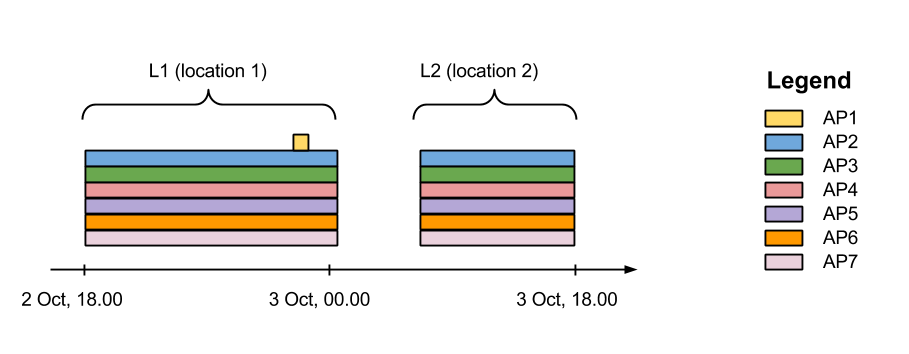
\includegraphics[height = 0.35\textwidth]{figures/isolated_ap.png}
\caption{Example of an isolated observable access point}
\label{isolated_ap}
\end{figure}

The above scenario considers a very small number of access points and a very
short period of time. The time gains in eliminating the access point which does
not provide so much information in this case would be very small. However, If we
are, for example, looking at a month of collected data for a user, we will have
entries for thousands of different access points that were observable at any
moment during this time. Out of these entries there can be hundreds of access
points which are never visible to the device during close scans and as such
their importance when determining the fingerprints for the different locations
is very limited, yet they do have a huge impact on the execution time needed to
actually extract the locations.

In order to solve this issue, we eliminate from the access points those ones who
are not respecting the following condition:
\begin{itemize}
  \item There is no time window of at least 5 minutes throughout the time
  duration of the analyzed data in which the access point has appeared for at
  least 5 times. %TODO - think about 5 times or 3 times and justify
\end{itemize}

% TODO - justify 5 minutes
We have chosen to use time windows of 5 minutes as we make the assumption that
any user will choose to spend minimum 5 minutes at each stop location. In case
the user spend less time, we can consider that they are just transitioning until
the next stop location.
